\documentclass[12pt,a4paper]{article}
%\usepackage[in]{fullpage}
\usepackage[utf8x]{inputenc}
\usepackage{cite}
%\usepackage{listings}
\usepackage[usenames]{xcolor}
\usepackage{graphicx}
\usepackage{hyperref}
\usepackage{xr} % cross-reference across files
\usepackage{float} %for H positioning

\externaldocument[TUT-]{tutorial}

% start a new section on a new page
\let\stdsection\section
\renewcommand\section{\newpage\stdsection}

%\lstset{ %
%  basicstyle=\footnotesize,        % the size of the fonts that are used for the code
%  breakatwhitespace=true,          % sets if automatic breaks should only happen at whitespace
%  breaklines=true,                 % sets automatic line breaking
%  commentstyle=\color{gray},    % comment style
%  keepspaces=true,                 % keeps spaces in text, useful for keeping indentation of code (possibly needs columns=flexible)
%  language=bash                 % the language of the code
%}

%opening
\title{CTA user manual}
%\author{Roger Biffiger, PSI}
\date{}

\begin{document}

\maketitle

\version{This user manual has been generated from the CTA src tree version 1.0.3}

%\begin{abstract}
%\end{abstract}

\tableofcontents

%\newpage

\section{Introduction}\label{sec:Introduction}
This is the user manual for the CTA (Complex Triggering Application).
The CTA allows a user to define a sequence of events and to distribute
these events to the event receivers in a subtree of a MRF (Micro
Research Finland) based timing system. In SwissFEL CTA is used in the
experimental stations ESA and ESB.

\section{Overview}\label{sec:Overview}
A timing system build from MRF hardware components has a tree topology.
There is one master at the root of the tree which generates the timing
stream signal. There are fanouts at each
crotch to multiply the number of ports providing a timing stream signal.
Finally there are event receivers at the leafs of the tree which receive
the timing stream, decode it and produce pulses on physical outputs
to trigger devices.
A simplified timing system tree can be seen in Figure \ref{fig:tim_sys_tree}.

\begin{figure}[H]
	\centering
	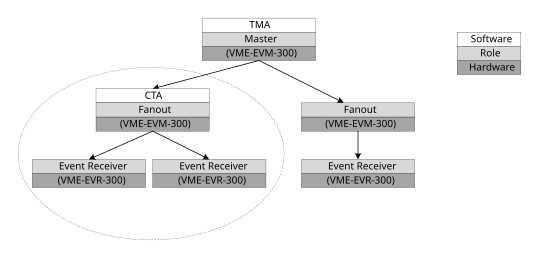
\includegraphics[width=\columnwidth]{./img/overview_1}
	\caption{Simplified timing system tree}
	\label{fig:tim_sys_tree}
\end{figure}

The decision which event code is distributed with what delay in each machine
pulse is done by the two EPICS software applications TMA (Timing Master
Application) and CTA (Complex Triggering Application).

The TMA runs on the master and has the following responsibilities:
\begin{itemize}
\item
Provide a set of PVs to the operator which allows the operator to control
the timing of the accelerator.
\item
Based on the operator PVs, the TMA must compute the sequence of events which
is to be send out in the next machine pulse.
\item
The TMA must write the event sequence to the hardware which writes it
to the timing stream.
\end{itemize}

The CTA is an EPICS software application which runs on a fanout. It has the
following responsibilities:
\begin{itemize}
\item
Provide a GUI which allows the user to define a sequence of event codes.
\item
The GUI must be able to download the event code sequence to the IOC
running the CTA.
\item
The CTA must program the hardware such that the sequence of event codes
is send in the timing stream.
\end{itemize}

Refer to section \ref{sec:Examples} for examples how an event code sequence
is injected in a timing stream signal.

TMA event codes are seen by all event receivers in the tree. CTA event
codes are seen by event receivers in the CTA subtree only.
In SwissFEL we use the CTA for the ESA and ESB timing subtrees.
To avoid interference of TMA and CTA event codes we decided to separate the
TMA and CTA event codes in event code space and time.
\begin{itemize}
\item
Event codes from 200-219 are reserved for CTA events. The TMA will not
use these event codes.
\item
The delay of CTA event codes is between 100-233 us. The TMA will not send event
codes with this delay.
\end{itemize}
ESA CTA event codes can not interfere with ESB CTA events codes because the
subtrees are on separate branches of the timing tree.

CTA event codes have a fixed delay. The delay value for each CTA event code
can be seen in table \ref{tab:cta_event_delays}

\begin{table}[!hbt]
\caption{Delay of CTA event codes}
\label{tab:cta_event_delays}
\centering
  \begin{tabular}{|c|c|}
    \hline \textbf{event code} & \textbf{delay [us]} \\ \hline
    \hline 200 & 100\\
    \hline 201 & 107\\
    \hline 202 & 114\\
    \hline 203 & 121\\
    \hline 204 & 128\\
    \hline 205 & 135\\
    \hline 206 & 142\\
    \hline 207 & 149\\
    \hline 208 & 156\\
    \hline 209 & 163\\
    \hline 210 & 170\\
    \hline 211 & 177\\
    \hline 212 & 184\\
    \hline 213 & 191\\
    \hline 214 & 198\\
    \hline 215 & 205\\
    \hline 216 & 212\\
    \hline 217 & 219\\
    \hline 218 & 226\\
    \hline 219 & 233\\
    \hline
  \end{tabular}
\end{table}

\section{GUI}\label{sec:GUI}
\subsection{Starting the GUI}
The GUI to control the CTA can be started on a console with the following
command:
\begin{itemize}
\item
ESA: start\_cta\_gui.sh ESA SAR-CCTA-ESA
\item
ESB: start\_cta\_gui.sh ESB SAR-CCTA-ESB
\end{itemize}

\subsection{Using the GUI}
The GUI can be used for the following tasks:
\begin{itemize}
\item
Down/upload a sequence to/from the IOC. 
\item
Define or modify a sequence.
\item
Start the sequence on the IOC.
\end{itemize}

\begin{figure}[H]
	\centering
	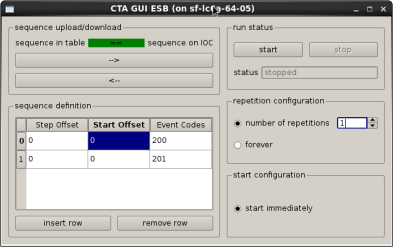
\includegraphics[]{./img/gui_1}
	\caption{CTA GUI}
	\label{fig:output}
\end{figure}

\paragraph{sequence upload/download:}
The widgets in the section \emph{sequence upload/download} can be used
to upload the sequence from the IOC to the sequence definition table
or to download the sequence in the sequence definition table to the IOC.
A widget indicates whether the sequence in the sequence definition table
and the sequence on the IOC are equal or not.

\paragraph{sequence definition:}
The section \emph{sequence definition} contains the sequence definition
table. Each line in the table defines an event code which is to be distributed
in a certain machine pulse.
The \emph{Step Offset} and \emph{Start Offset} columns define
the machine pulse. The column \emph{Event Code} defines the event code.
The \emph{Step Offset} can be used to define the machine pulse for sending
relative to the last line and the \emph{Start Offset} can be used to define
the machine pulse for sending relative to the first line.
If the user enters a \emph{Step Offset} the \emph{Start Offset} is
set automatically and vice versa.
There are buttons to insert and remove new lines. This can also be
done with the context menu.

\paragraph{start configuration:}
The radio buttons in the \emph{start configuration} section can be used to
define when CTA starts distributing the sequence on the IOC.
Currently the only option is \emph{start immediately}. If this option is selected
the CTA starts sending the event sequence immediately. The time between
pressing the start button and the time the first event code is send
is short but undefined.

\paragraph{repetition configuration:}
The radio buttons in the \emph{repetition configuration} section can be used
to define how many times the sequence is repeated.

\paragraph{run status:}
The widgets in the \emph{run status} section can be used to start or stop
event code sending of the CTA. The \emph{status} widget shows the current
status of the CTA.

\section{Sequence definition examples}\label{sec:Examples}
This section provides some examples of CTA GUI configurations together
with the resulting sequence of event codes.

\subsection{One local sequence started immediately}\label{subsec:one_seq_imm}
\begin{figure}[H]
	\centering
	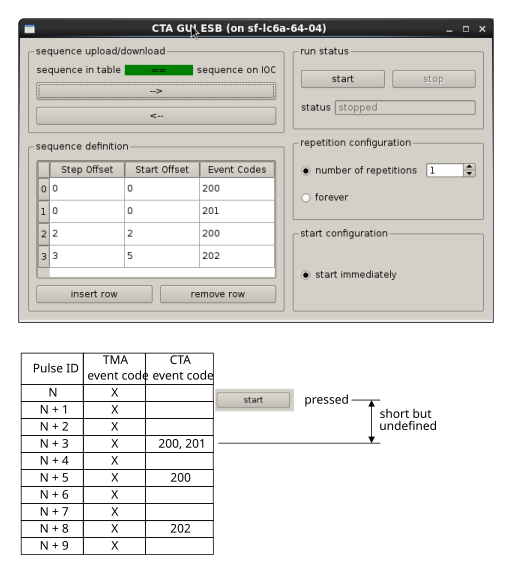
\includegraphics[width=\columnwidth]{./img/ex_single_seq_1}
	\caption{GUI and resulting event code sequence}
	\label{fig:pulser_generic}
\end{figure}


\end{document}
